
\section{Examples}\label{sec:examples}

% 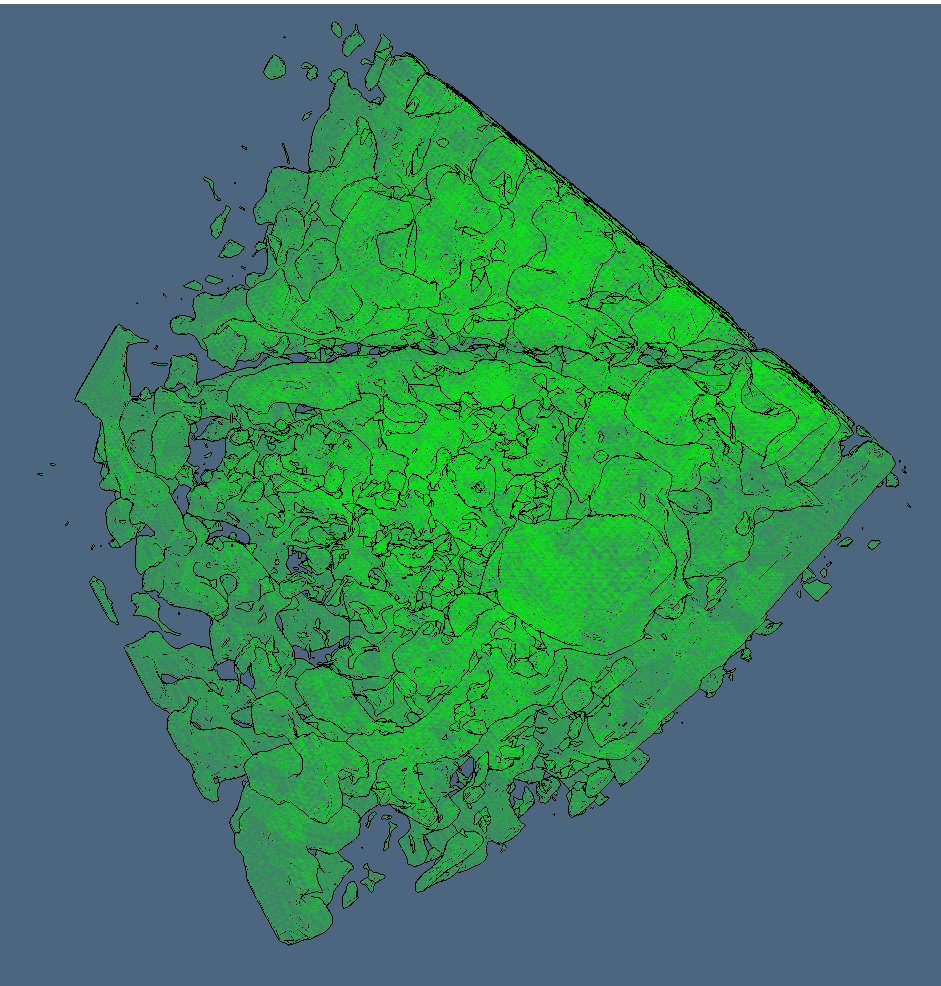
\includegraphics[height=0.3\textwidth]{figs/nrn10_100_green.png} 
%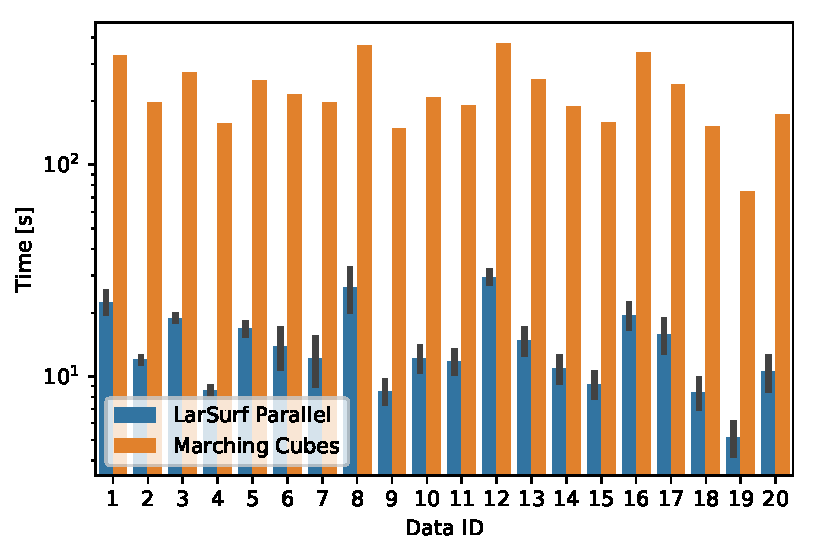
\includegraphics[scale=1]{input/ircad_comparison.pdf} 

\begin{figure}[tbp]
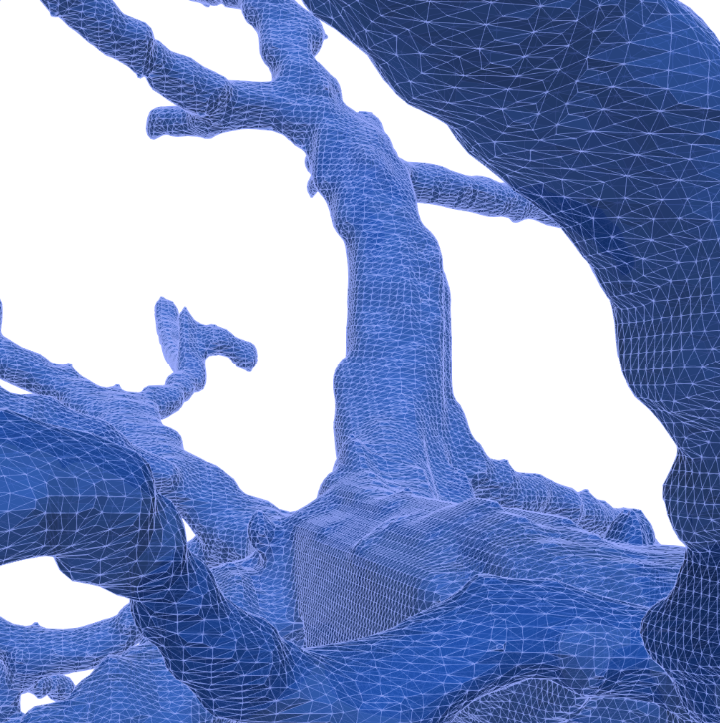
\includegraphics[height=0.3\textwidth,width=0.33\textwidth]{figs/image-1.png}%
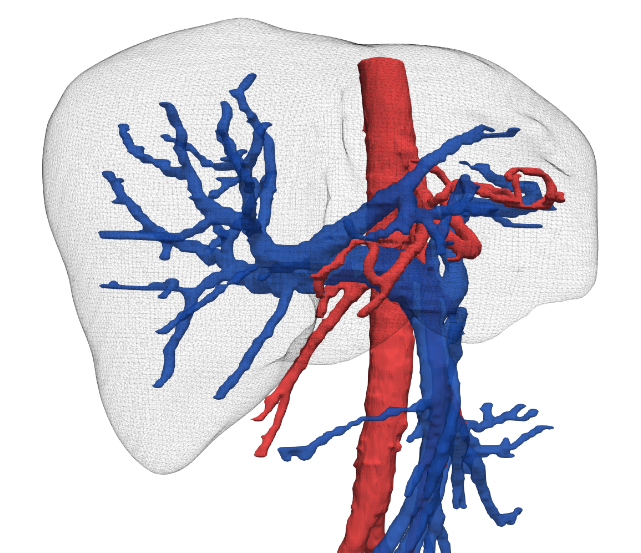
\includegraphics[height=0.3\textwidth,width=0.33\textwidth]{figs/image-2.png}%
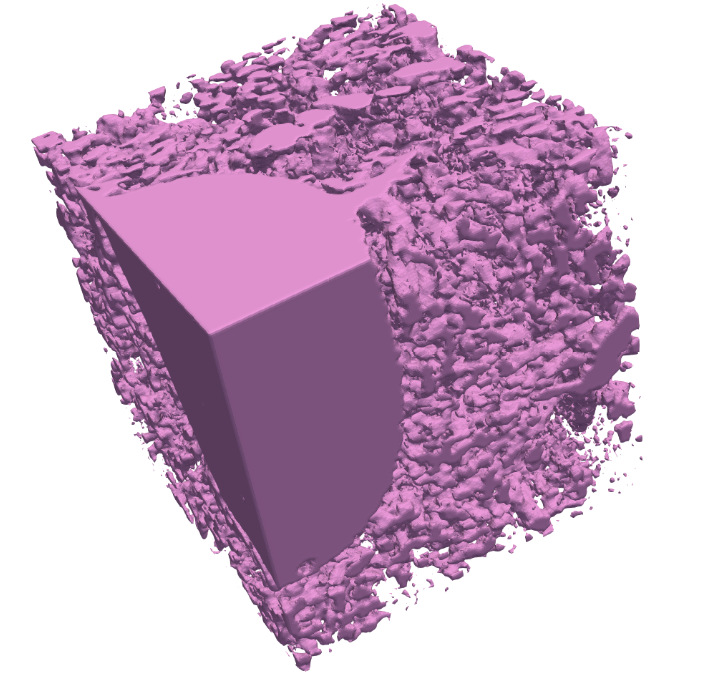
\includegraphics[height=0.3\textwidth,width=0.33\textwidth]{figs/image-3.png}%
\caption{\small Triangulated surfaces of the macroscopic and microscopic structures of the liver extracted by the \textsc{lar-surf} algorithm. 
(a) Detail of the portal vein (PV) with resolution $1.6\times0.57\times0.57$ $[mm]$.
(b) model of the human liver, with portal vein and hepatic artery connected to colon and stomach.
(c) microvasculature of a pig liver, based on corrosion cast of interlobular veins prepared by Eberlova
\cite{eberlova2017use}. The size of the specimen is 0.936 $[mm]$ along each axis and the resolution of the Micro-CT data is 4.682 $\mu{}m$. Note that brick boundaries are flat.
}
\label{fig:example_liver_macro_micro}
\end{figure}

%\begin{figure}
%\centering
%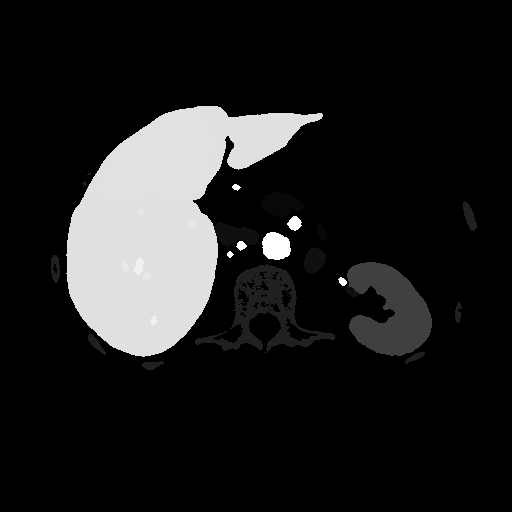
\includegraphics[width=0.40\textwidth]{figs/ircad01_segmentation_65.png}
%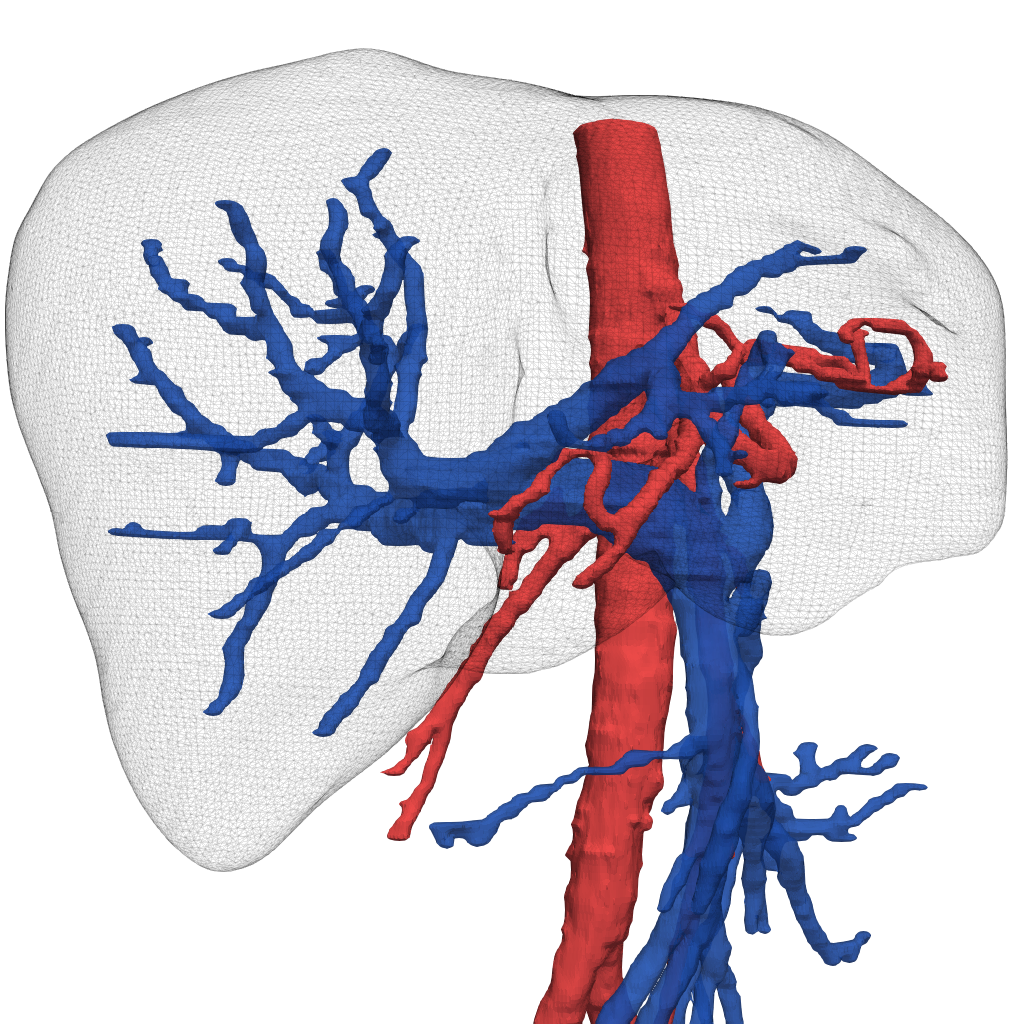
\includegraphics[width=0.40\textwidth]{figs/ircad01_liver_tricolore_01.png}
%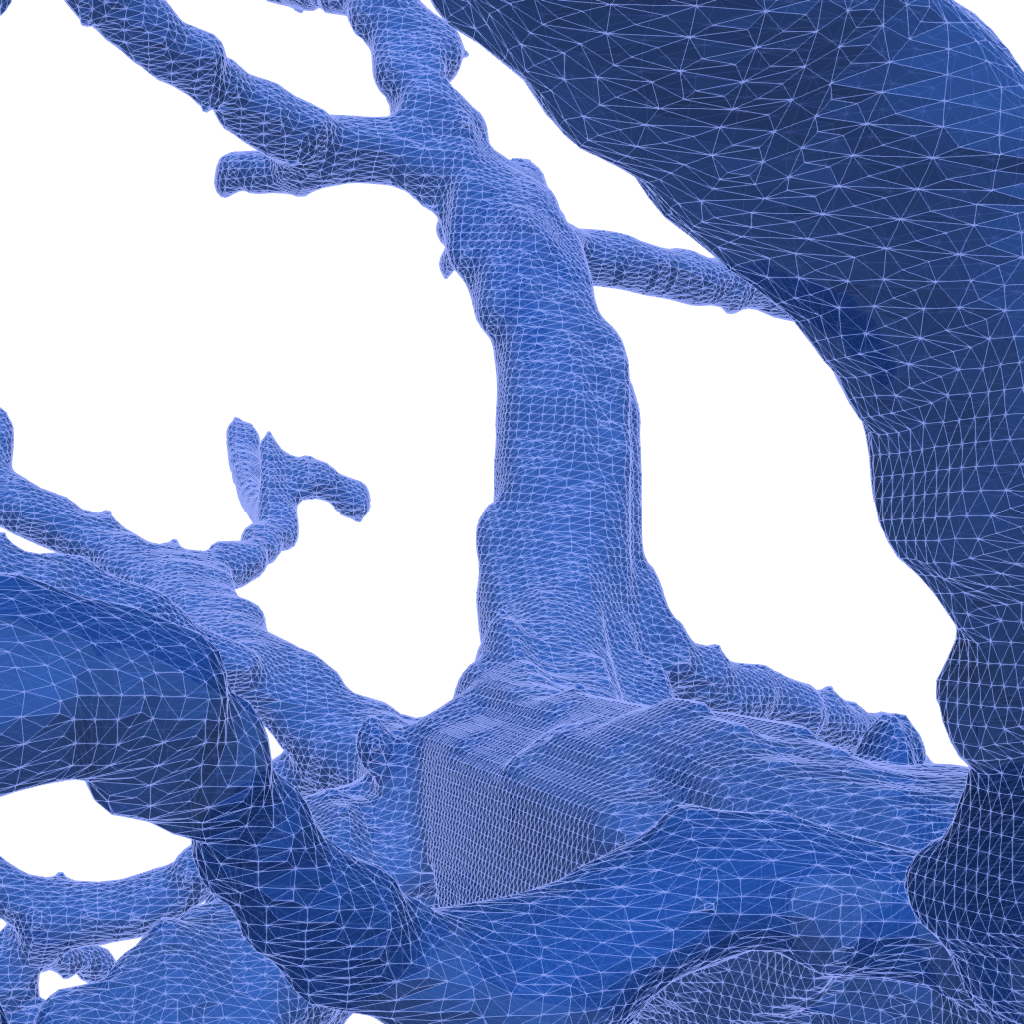
\includegraphics[width=0.40\textwidth]{figs/ircad01_porta_blue_01.png}
%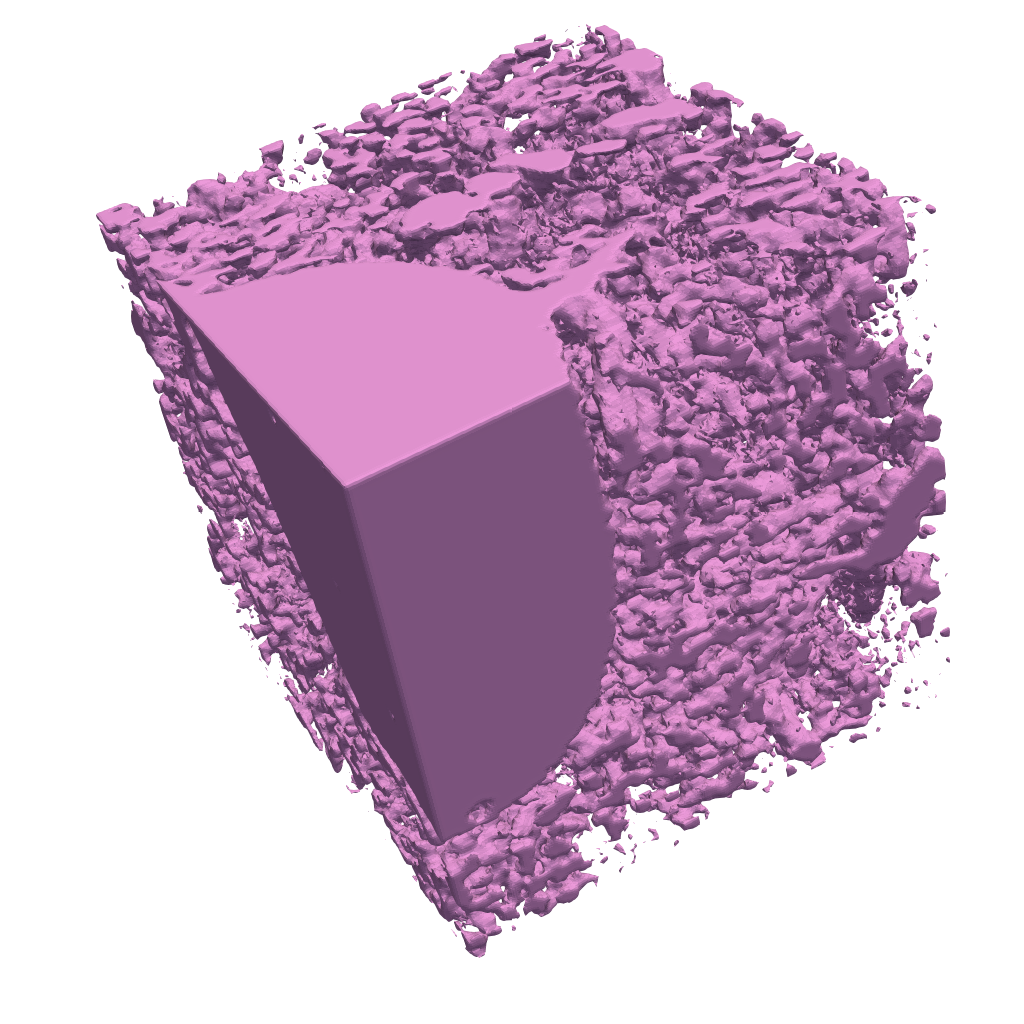
\includegraphics[width=0.40\textwidth]{figs/nrn10_200_pink_02.png}
%% 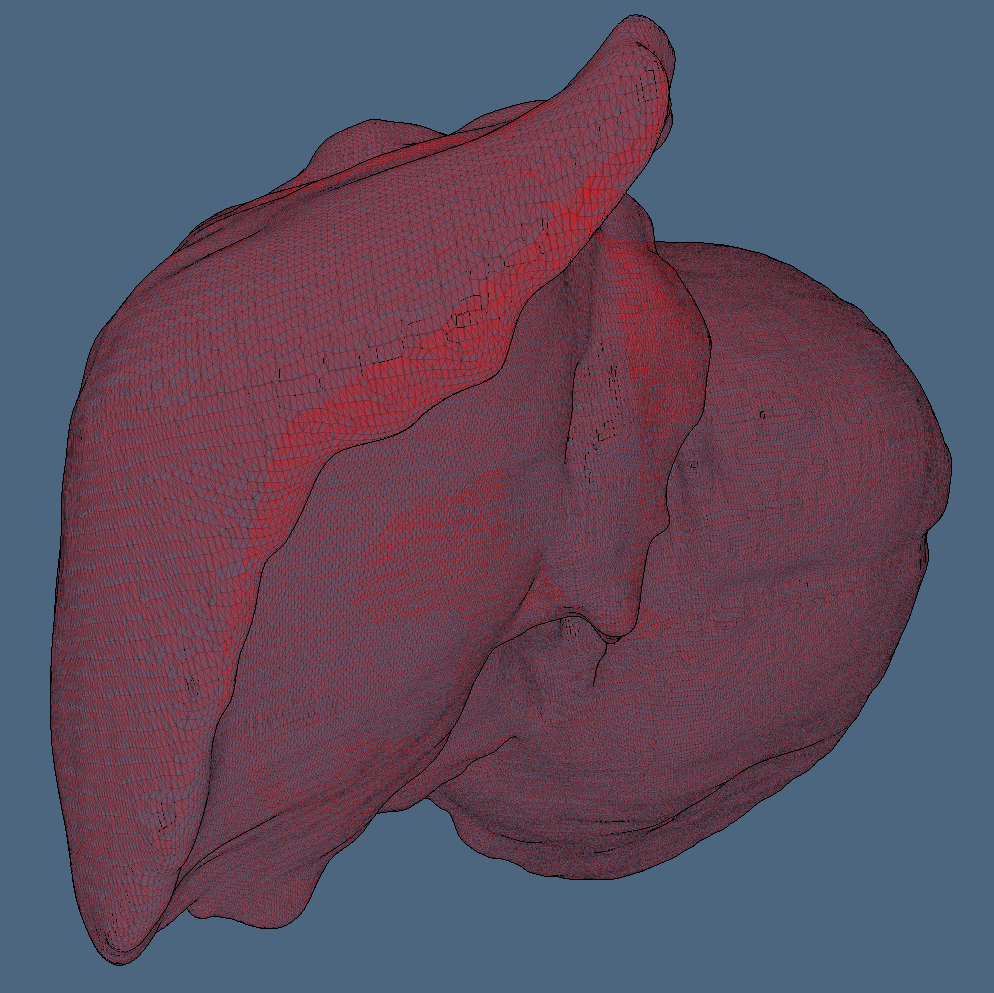
\includegraphics[width=0.4\textwidth]{figs/liver_01_red_3.png} 
%% % \vspace{0.05\textwidth}
%% 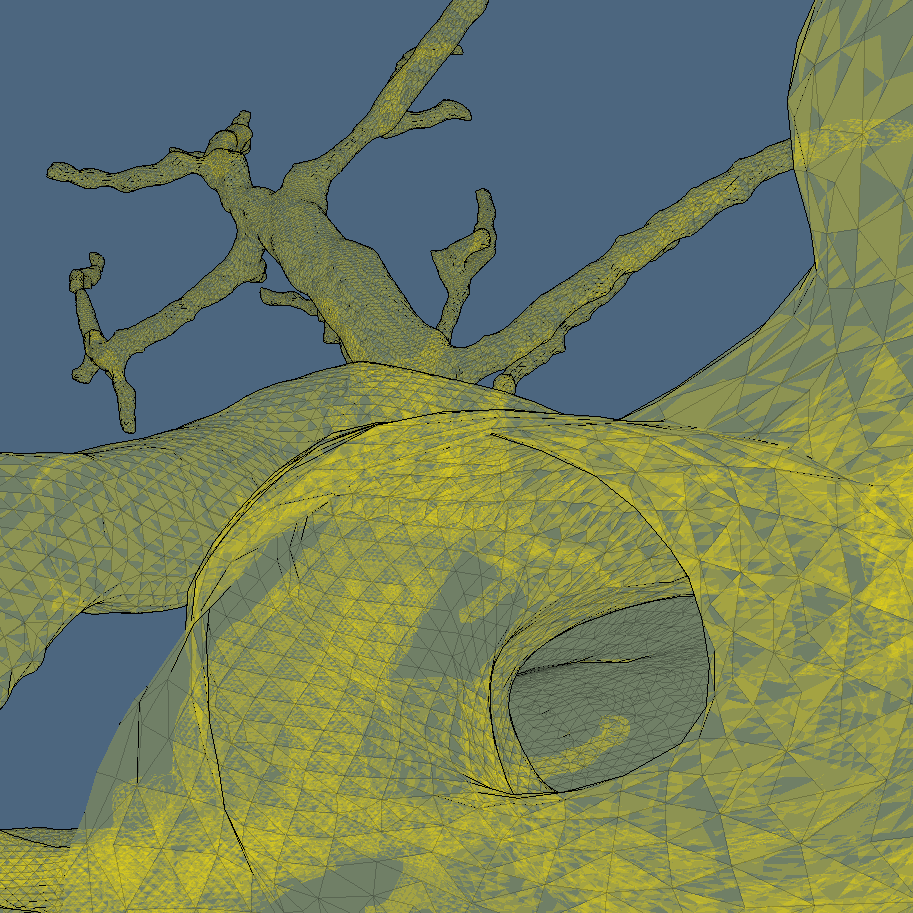
\includegraphics[width=0.4\textwidth]{figs/portalvein_01_yellow_3.png} 
%% % \vspace{0.01\textwidth}
%% 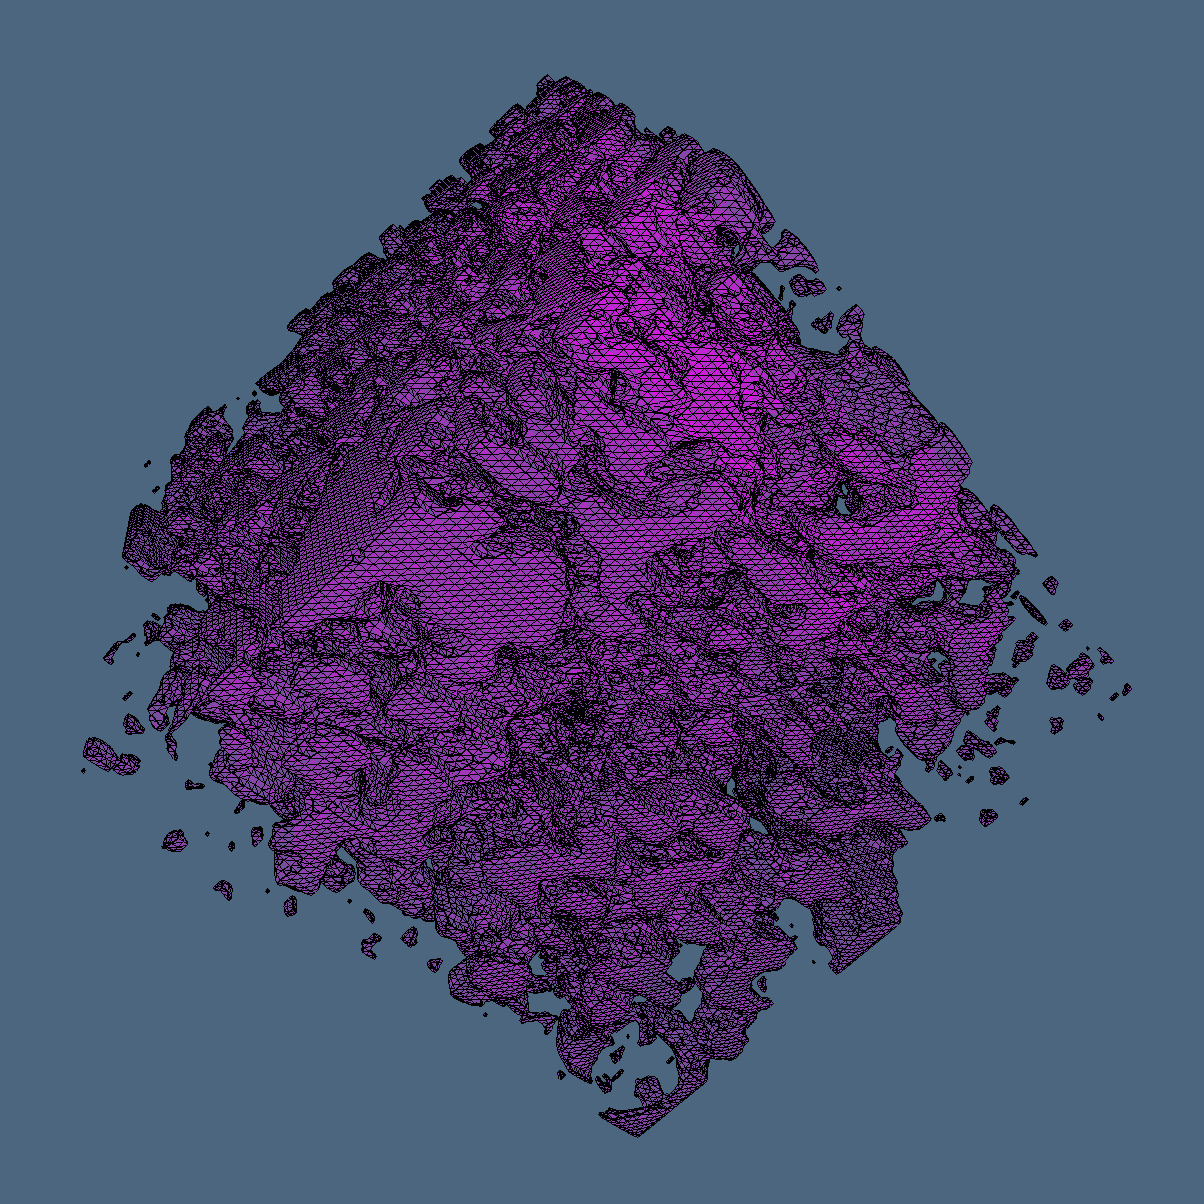
\includegraphics[height=0.4\textwidth]{figs/nrn10_100_magenta_high_res.png} 
%% % 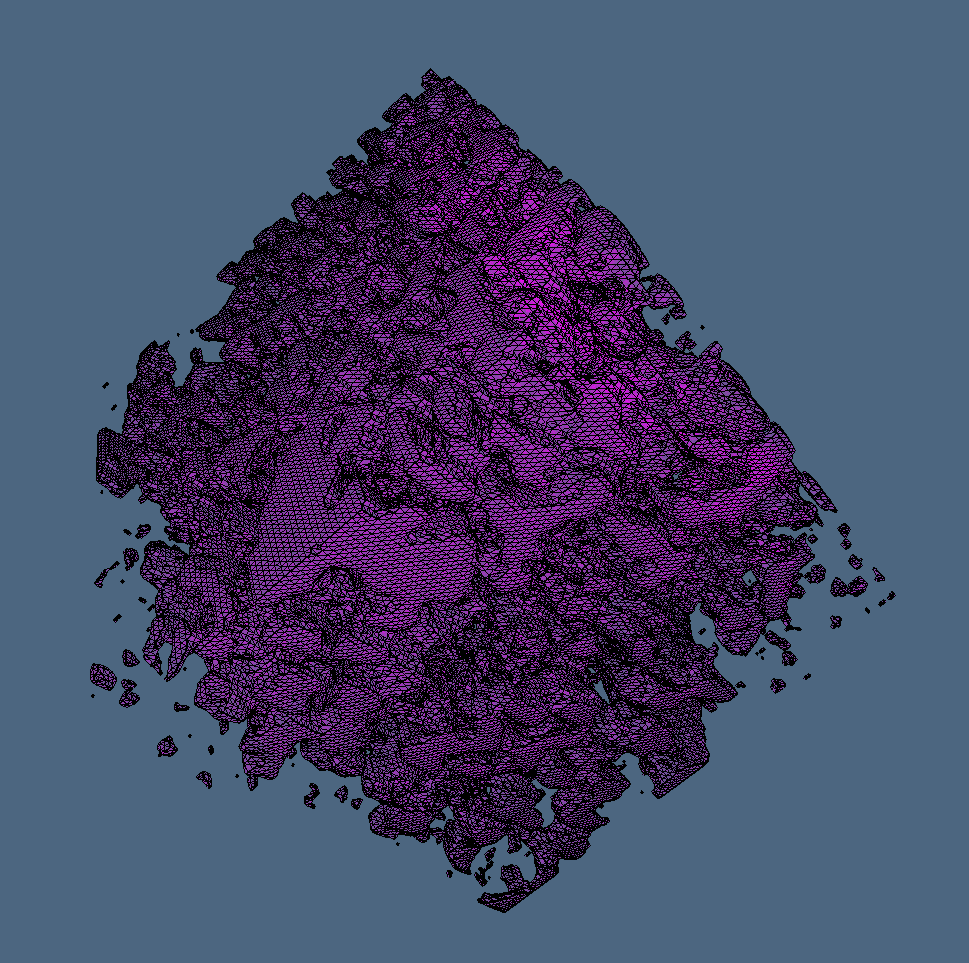
\includegraphics[height=0.4\textwidth]{figs/nrn10_100_low_res.png} 
%% % \vspace{0.05\textwidth}
%% 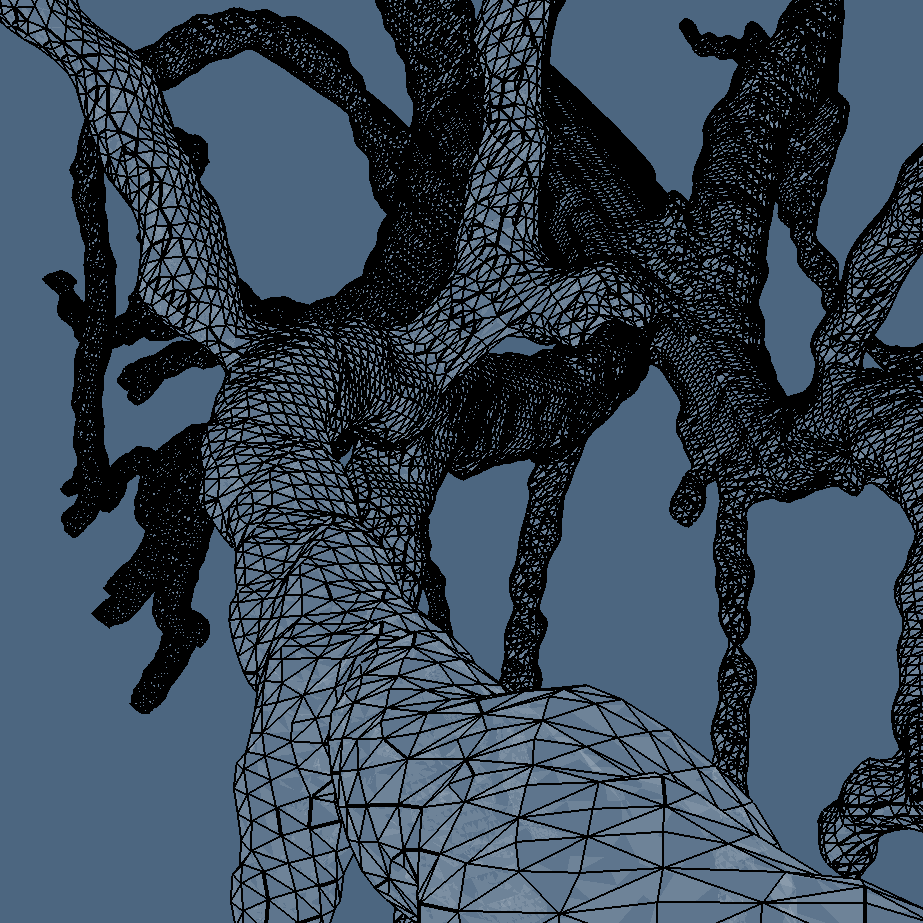
\includegraphics[width=0.4\textwidth]{figs/porta_smoothing_2.png} 
%\caption{
%Liver structures. The upper left image shows one slice  with segmented organs from  the Ircad dataset \cite{ircadb}.
%The other images show the triangulated isosurfaces of the macroscopic and microscopic structures of the liver extracted with \textsc{lar-surf} algorithm. 
%The wireframe model of the human liver along with the portal vein and hepatic artery can be seen on the upper right image. 
%The left bottom image shows the detail of the portal vein  
%with resolution $1.6\times0.57\times0.57$ $[mm]$.
%On the bottom right image is shown the microvasculature of a pig liver based on corrosion cast prepared by Eberlova
%\cite{eberlova2017use}. The size of the specimen is 0.936 $[mm]$ along each axis and the resolution of the Micro-CT data is 4.682 $\mu{}m$.
%} \label{fig:example_liver_macro_micro}
%\end{figure}
% Both right images show the Portal Vein from the same Ircad dataset \cite{ircad} 

% \begin{figure}
% \centering
% 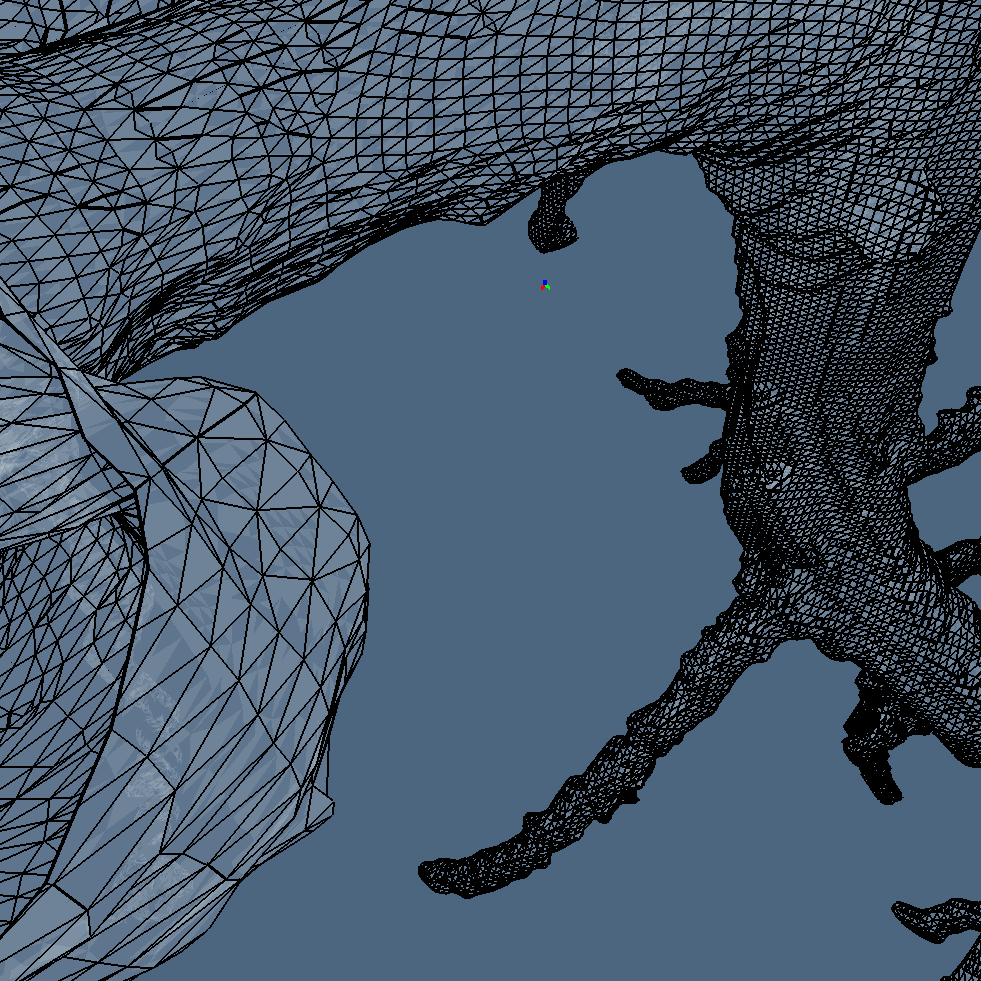
\includegraphics[width=0.4\textwidth]{figs/porta_smoothing_1.png} 
% \vspace{0.05\textwidth}
% 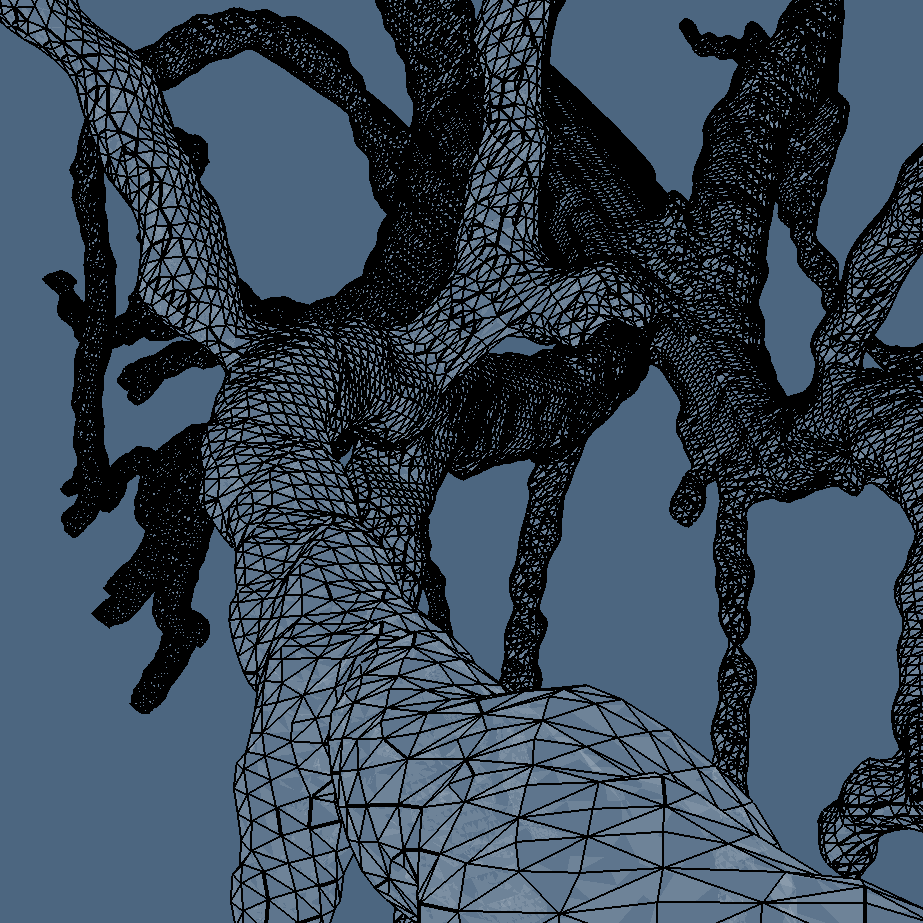
\includegraphics[width=0.4\textwidth]{figs/porta_smoothing_2.png} 
% %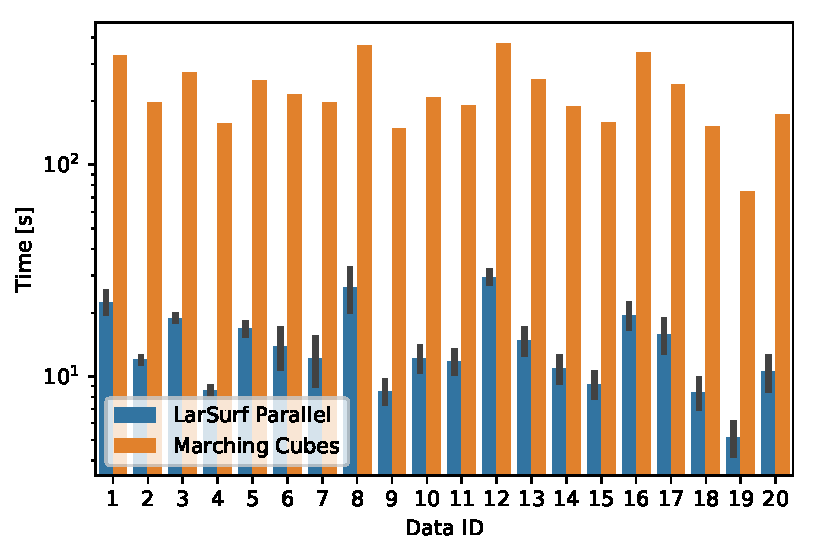
\includegraphics[scale=1]{input/ircad_comparison.pdf} 
% \caption{Triangulated isosurface of portal vein calculated with LAR-SURF}
% \label{fig:example_porta}
% \end{figure}

% The implementation of our algorithm is available in LarSurf package. 
Use of the \texttt{LarSurf.jl} package can be seen on listings \ref{lst:example1} where the liver segmentation with 2865131 voxels from the
Ircad dataset is used as an input for our surface extraction algorithm. The size of 3D volumetric 
image is $129 \times 512 \times 512$
and the voxel resolution is $1.6\times0.57\times0.57$ [mm]. 
The output liver surface model is formed by  182124 triangles and the number of vertices is 90822. 
The visualization can 
be seen in Fig. \ref{fig:example_liver_macro_micro}. 


\begin{lstlisting}[caption={Get surface from DICOM volumetric data}, label={lst:example1}, basicstyle=\small]
using Distributed
using Pio3d  # Read 3D data from DICOM files
addprocs(3)  # set number of processors
using LarSurf

LarSurf.lsp_setup([64, 64, 64])  # set block size

# read data from DICOM files
datap = Pio3d.read3d("3Dircadb1.1/MASKS_DICOM/liver")
segmentation = datap["data3d"]
voxelsize_mm = datap["voxelsize_mm"]

# get surface
V, FV = LarSurf.lsp_get_surface(segmentation, voxelsize_mm)
FVtri = LarSurf.triangulate_quads(FV)

# do smoothing and save data
Vs = LarSurf.Smoothing.smoothing_FV_taubin(V,FV,0.5,-0.2,40)
objlines = LarSurf.Lar.lar2obj(Vs, FVtri, "liver.obj")
\end{lstlisting}

The portal vein surface extraction can be performed with a small change of the input path in the code.
The 3D image resolution is the same. 
% It can be seen in the same figure. 
The number of input voxels is 103533. 
The output surface is created by 90822 vertices and 182124 triangles. 

The right image of Fig. \ref{fig:example_liver_macro_micro} is the surface of the microvasculature of a pig liver. 
The volumetric image is based on Micro-CT data of corrosion casts of pig liver.
\cite{eberlova2017use}.
The size of the visualized data is $100\times100\times100$ voxels and the size of the voxel is 4.682 $\mu{}m$.
The number of triangles is 
544784 and the number of vertices is 272826.

% \begin{minted}{python}



% using Pkg
% \end{minted}
% \begin{minted}[breaklines,escapeinside=||,mathescape=true, linenos, numbersep=3pt, gobble=2, frame=lines, fontsize=\small, framesep=2mm]{julia}
% Your awesome julia code here\end{minted}

\section{Discussion of method}\label{sec:discussion}

Most other methods for extraction of boundary surfaces from 3D data arrays---including~\cite{10.1016/j.cad.2006.09.003} and~\cite{10.1115/1.2960489}---use implicit functions, defined by first averaging upon 3D mesh vertices the lighting or brightness of incident voxels, and then by applying some marching cube algorithm in order to traverse and to triangulate  the iso-valued boundary patches.  

We use instead, we use a binary labeling of the voxel sets of the image segment of interest, and the standard medical 3D image array as solid representation. The set of boundary facets is extracted through spMV (sparse matrix vector multiplication) of the $[\partial_3]$ matrix times the binary vector labeling the voxels of the segment. The boundary matrix is computed once and for all, sent to all workers (cores or nodes), then used in parallel for all image brick extractions. This algebraic method can be immediately extended to multi-material processing, as well as to designing multi-material tissue layering for 3D printing.

In particular, we might organize a multi-material (or multi-organ) extraction, simply by multiplication of the boundary matrix $[\partial_3]: C_3\to C_2$  times a binary matrix where the non-zero elements on each column represent either one of the materials, or one of the organs to be algebraically extracted by the filter. The two surface patches common to two adjacent segments will be exactly coincident, and share the same geometry and topology, with the only exception of the each patch contours, where the influence of adjacent patches induces each instance to be separated and rounded-off.
%
%To make our algorithm consistent with results given by~\cite{10.1016/j.cad.2006.09.003} and ~\cite{10.1115/1.2960489} about the boundaries common to multiple patches is easy: (1) extract the 1-skeleton of the set of patches, using the boundary matrix $[\partial_2]: C_2\to C_1$ \emph{before} the rounding of surfaces; (2) make the resulting 1-chains curved and smooth, by 1D Taubin algorithm, (3) block their vertices before the Taubin smoothing of incident patches.

The main advantage of the approach discussed in this paper is given by its very algebraic nature; our implementation does not need any kind of algorithmic graph traversal, of difficult parallelization, but only the execution of standard algebraic computing kernels, and in particular the spMV and the spMspM (sparse matrix--sparse matrix multiplication) kernels, nowadays efficiently implemented by tensor processors on Nvidia hardware.  As we have shown, the parallelization, both shared-memory and distributed, is also fairly easy and with good speed-up.



